\section{Kentico CMS} \label{analysisKenticoCMS}
Kentico CMS \cite{kentico-product-overview} is a content management system (CMS) which allows clients to create and manage their web-sites using a single user interface (UI) which is made of tiles, a layout and an edit button. Each tile has its own functionality. The client can rearrange them either by simply dragging them or by pressing the edit button. Pressing the button leads to the tiles having an \textit{X} in the upper-right corner for removing the tile. If place on the dashboard is available, a blank rectangle with a plus in the position of the future tile enables the client to add a new tile from the menu. 

\begin{figure}[ht!]
  \centering
  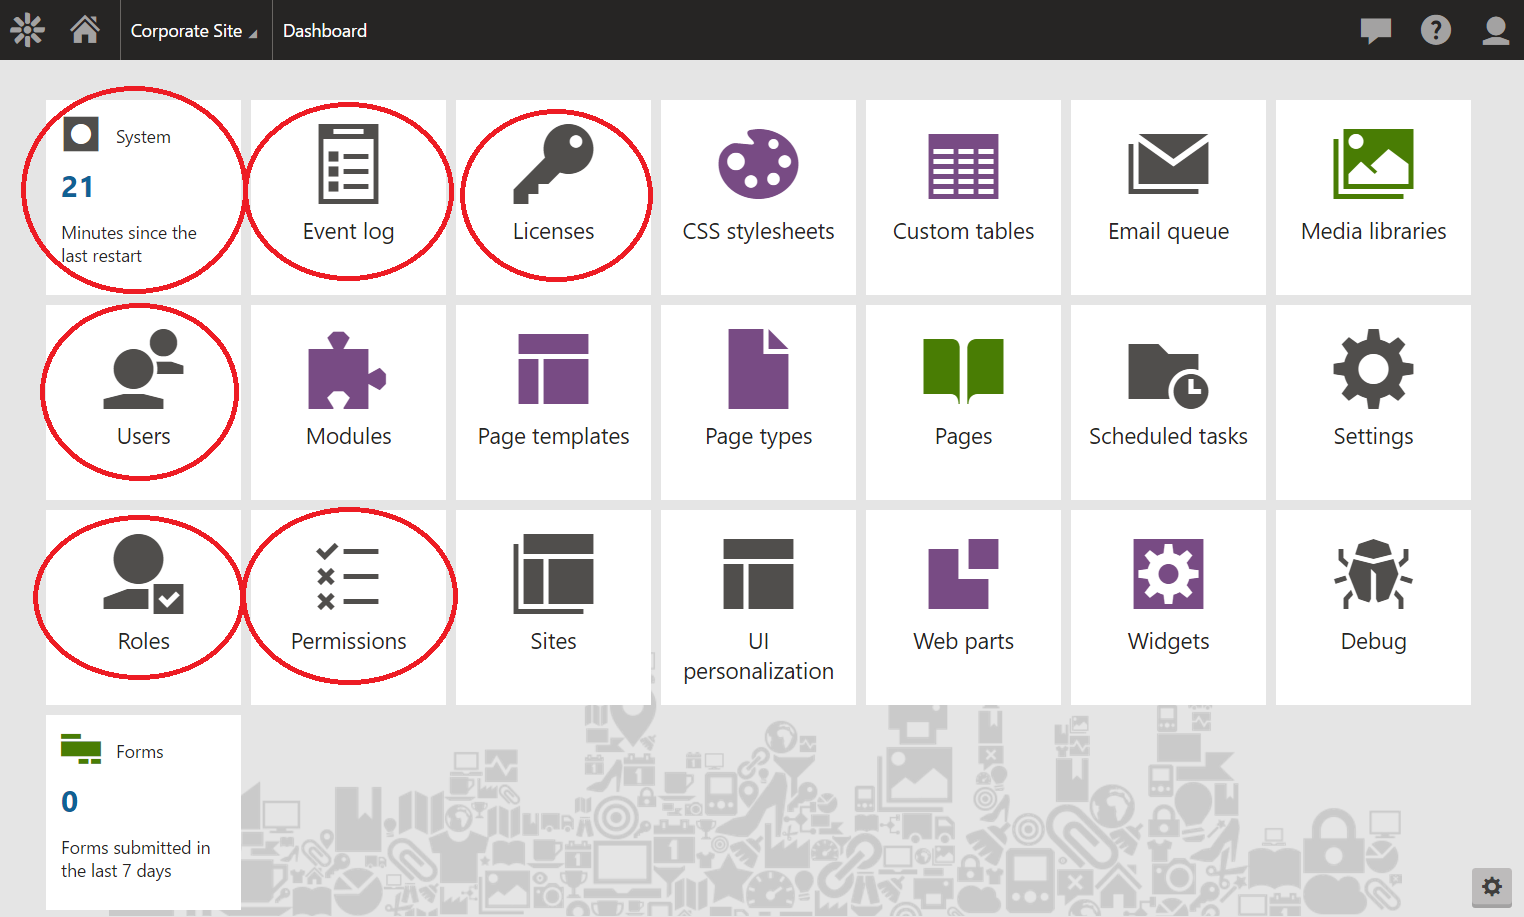
\includegraphics[width=\textwidth]{Images/Kentico9.png}
  \caption{Kentico 9.0 UI. The functionality of the tiles in the red circle is implemented in the KenticoApp. This image was
taken via print screen from the administration interface of the Kentico 9.0 product and was modified for illustrational purposes.}
  \label{kentico9UI}
\end{figure} 

The functionality in the menu is divided into six categories, namely: Content Management, On-line Marketing, E-Commerce, Social \& Community, Development and Configuration. 
\begin{description}
\item [Content Management] sees to the contents of the client's site such as pages, tables, polls, etc. 
\item [On-line Marketing] enables the client to handle marketing elements. Visitor's behaviour and reactions are taken into consideration. The tiles to be chosen are Email marketing, MVT Tests, Personas and others. 
\item [E-commerce] offers actions which lead to motivating the visitor's behaviour to resemble the client's wished one, managing products and to track sales. These action are for example Buy X get Y discounts, Products and Store reports. 
\item [Social \& Community] makes it possible for the client to maintain the community around the site and its communication. Some of these tiles are for instance Avatars, Chat, Events. 
\item [Development]'s task is to empower the client to administer sources of functionality and programmable elements. This section consists of tiles such as CSS stylesheets, Email templates, Web Part Containers, etc. 
\item [Configuration] The last, in this thesis most important category. This category mostly oversees the overall configuration of the Kentico server. It contains the key requirements of KenticoApp.
	\begin {description}
	\item [System] One of those requirements is the System tile. Part of the System are several subcategories. The one of interest, however, is the one called General. It shows general information about the system and system time, the database and statistics of memory, garbage collection, cache and page view. The default value of the refresh interval is 1 second. It can be changed to up to 60 seconds. Other services General provides are Restart application, Clear cache, Clear performance counters and Clear unused memory. 
	\item [Eventlog] is another key feature. It offers a dropdown list of available sites, a list of events, a filter to view specific events and a button to clear the log. 
	\item[Licenses] the purpose of tile is to show and add licenses of the client and their details. It also allows the client to Export list of domains. 
	\item [Users] grants the ability to view, add and edit the users, monitor the on-line ones and send mass emails. A filter tool is at service for searching users.
	\item [Roles] Users are assigned with roles and this is where these roles are administered. The overview displays all of the site's roles end their details. The client is able to add, edit and delete roles. A dropdown with sites to be chosen is present. 
	\item [Permissions] Roles authorize users to execute certain actions. Permissions define what these actions are. They are managed in this tile. Again, filter options and a dropdown with site names are available. 
	\end{description}
\end{description}
More functionality can be added to the Kentico application by using already created modules or by developing new ones from scratch since it is an extensible system.

\section{Web API} \label{analysisWebAPI}
An~API is a~collection of~functionality which a~programmer is able to~utilise in a~third party app. A web API is an API intended for utilisation by a web server or browser.
\subsection{REST} \label{analysisREST} \cite{rest}
REST is an architecture of client-server communication. APIs built using this architecture utilise most commonly JSON format and are lightweight. This means they operate with simple data representation and therefore the delay between sending and delivering is comparatively small. The client needs no knowledge of how the server is built. It depends on the resources (nouns) and operations (verbs). Hyper text transfer protocols (Http) status codes (SC) can be returned after executing the verbs. The nouns are identified with Universal Resource Identifiers (URIs). Each URI represents only one noun. The system returns a SC depending on the success of the call and if unsuccessful according to the reason why the call was unsuccessful. Some of the most common SCs are described below\cite{rfc-2616}.
\begin {description}
\item [200 OK] SC means the request was successful and the data have been returned. SC \textit{204 No Content} represents the same meaning but returns nothing.
\item [201 Created] is used when the request was successful and the resource was created. It should return a link to the resource created.
\item [400 Bad Request] is returned when the given parameters were invalid. A reason might be added in the error message. The call should be repeated with different parameters.
\item [401 Unauthorized] it transmits the information the user should try and sign in again. It is meant to be returned if the client is not signed in or does not have the needed permissions. However, it mostly is returned if the user is not authenticated.
\item [403 Forbidden] its purpose is to let the user know not to repeat the request. It is meant to be returned if the client is authorized and authenticated but the system refuses to execute the call but it is most often applied in case the client is not authorized to execute a specific call.
\item [404 Not Found] is shown if a resource is not found with the given URI and it is unknown how long this condition will remain. It can be used if the reason for the failure remain unknown or a resource has to be hidden. Also this is the SC which is applied if no other code is suitable.
%\item [500 Internal Server Error] is returned if the server failed the call due to an unexpected event. 
\item [503 Service Unavailable] SC means the server is not able to fulfill the request at the moment. It is utilised when maintaining the server or overloading it.
\end{description}	
The most applied verbs are described using the following keywords: \textit{OPTIONS}, \textit{GET}, \textit{POST}, \textit{PUT}, \textit{PATCH} and \textit{DELETE}. For the description of them we provided two example URIs:

\begin{enumerate}
\item 
\lstset{style=sharpc}
\begin{lstlisting}
http://example.com/students/47
\end{lstlisting}

\item 
\lstset{style=sharpc}
\begin{lstlisting}
http://example.com/students
\end{lstlisting}
\end{enumerate}

\begin {description}
\item [OPTIONS] offers information about what verbs can be invoked upon a noun. The first URI example with the prefix \textit{OPTIONS} returns all of the bellow verbs. 
\item [GET] is used to read data from the server. It is read only, data must not be changed. The SCs it returns are \textit{200}, \textit{400} and \textit{404}. The first URI example with the prefix \textit{GET}returns the student with the ID 47.
\item [POST] is mostly utilised to create data. It returns SCs such as \textit{201}, \textit{400} or \textit{404}. The second URI with the prefix \textit{POST} creates a new student and returns the resource's location.		
\item [PUT] is most commonly leveraged for updating resources with the sent data. The data are a representation of the complete resource. It returns SCs \textit{200}, \textit{204} and \textit{404}. The first URI edits the student with the id 47.
\item [PATCH] is mostly used for modifying resources. The difference between PATCH and PUT is the sent data can be described by only a part of the resource that needs to be changed. It returns the same SCs as \textit{PUT}. The first URI with the prefix \textit{PATCH} modifies the student with the ID 47.
\item [DELETE] deletes the resource. It returns the status codes \textit{200} and \textit{404}. The first example URI with the prefix \textit{DELETE} deletes the student with the id 47.
\end{description}
Each verb can be shared among multiple nouns. However, each noun might not be able to use each verb. For example an AT usually is not updated, therefore the verb \textit{PUT} is not used with the AT resource.

The server's and client's platform is not relevant. Which is the reason why REST is widely used in web apps. The session between the client and server is stateless, which means the server does not store the client's state. Instead it generates an AT which is send to the client. This is an advantage since the client is enabled to communicate with different servers or machines in one session. Another benefit is if the server has to be restarted no data of the client's state are lost. It also makes the system highly scalable. REST is an alternative to Simple Object Access Protocol (SOAP), which is more complicated. It has a steeper learning curve and, on initialisation, sends a file with the description of the architecture. It usually operates with Extensible Markup Language (XML). It is slower and heavier than REST. 

\section{Mobile applications} \label{analysisMobileApplications}
Mobile apps are more important every day since \textit{no other technology has impacted us like the mobile phone. It's the fastest growing manmade phenomenon ever -- from zero to 7.2 billion in three decades.}\cite{more-gadgets-on-earth-than-people} The platforms, on which these apps run on, can be divided into three main categories: Android, iPhone OS (iOS) and the Windows family of operating systems for mobile devices (WM). The most used operating system (OS) with a share of 68.67\% of all mobile devices as of November 2016, according to \textit{netmarketshare.com} \cite{operating-system-market-share} is Android. It was  released in September 2008 and its native language is Java. With a percentage of 25.71\%, iOS is the second most sold mobile OS and was released in June 2007. Its native language is Swift. The third platform is WM with 1.75\% share. It was first released in November 2010 and the native language is C\#. 

Mobile apps can be divided into three types: Native, HTML5 and Hybrid.
\begin {description}
\item [Native] This type of app is written in the native language of the platform the developer wants to target. It is fast and the behaviour is most intuitive for its users because the developer focuses on one particular OS and its features. The drawback is that for the development of a native app the learning curve is steep which is why an experienced team of programmers is needed and it targets only one OS. If the app has to run on other platforms, it has to be built in their native languages. This is time costly and therefore expensive. 
\item [HTML5] These apps run in a devices browser. They are usually implemented in CSS, HTML and JS. Many programmers have the opportunity to leverage their previously acquired experience with these languages, alternatively the skills gained here in web programming. HTML5 based apps run slower than native ones but work on multiple OS. This saves time and money. The disadvantage of cross-platform apps is they are less intuitive. For example an app with android features would be uncommon for iOS users and vice versa. Another flaw of this approach is the inability to use the device's hardware, such as its camera or microphone.
\item [Hybrid] This is a combination of the two above. It is primarily built utilising CSS, HTML5 and JS and is \textit{hosted inside a native application that utilizes a mobile platform’s WebView.} \cite{hybrid-mobile-app} The bridge to native technologies is ensured by tools, for example in this thesis the Apache Cordova framework (ACF) is used. A WebView is a headless browser, without any buttons and without higher level functionality such as tabs, navigation, etc. The perks of this approach is the small learning curve. Thanks to HTML5 it is cross-platform and the native wrapper allows it to use the device's hardware and native API. It still runs slower than Native but is cheaper when more OSs are targeted.
\end{description}

When creating an app the developer has to consider what approach will be the most effective one. If smooth graphical performance is crucial, the app should be native. If it has to run on multiple platforms, make use of a device's hardware component and native API and the graphics are not that important, probably hybrid would be the best fit. If the app displays what was sent to it and has no dynamic graphics then HTML5 should suffice.

